%%%%%%%% ICML 2018 EXAMPLE LATEX SUBMISSION FILE %%%%%%%%%%%%%%%%%

\documentclass{article}

% Recommended, but optional, packages for figures and better typesetting:
\usepackage{microtype}
\usepackage{graphicx}
\usepackage{subfigure}
\usepackage{booktabs} % for professional tables
\usepackage{listings}
\usepackage{xcolor}
\usepackage{enumerate}
\usepackage{appendix}
\usepackage{mdframed}
\usepackage{multirow}
\usepackage{bigstrut}
\usepackage{csquotes}
% hyperref makes hyperlinks in the resulting PDF.
% If your build breaks (sometimes temporarily if a hyperlink spans a page)
% please comment out the following usepackage line and replace
% \usepackage{icml2018} with \usepackage[nohyperref]{icml2018} above.
\usepackage{hyperref}

\colorlet{punct}{red!60!black}
\definecolor{background}{HTML}{F6F6F6}
\definecolor{delim}{RGB}{20,105,176}
\colorlet{numb}{magenta!60!black}

% Attempt to make hyperref and algorithmic work together better:
\newcommand{\theHalgorithm}{\arabic{algorithm}}
\renewcommand\lstlistingname{\vspace{1.5mm} Extract}
% Use the following line for the initial blind version submitted for review:
%\usepackage{icml2018}

% If accepted, instead use the following line for the camera-ready submission:
\usepackage[accepted]{icml2018}
\lstset{language=Python,   basicstyle=\tiny\ttfamily, backgroundcolor=\color{black!5!white}, breaklines=true}

% The \icmltitle you define below is probably too long as a header.
% Therefore, a short form for the running title is supplied here:
\icmltitlerunning{Natural Language Understanding - Recurrent Neural Networks Coursework}


\begin{document}

\twocolumn[
\icmltitle{NLU -- Recurrent Neural Networks Coursework}

% It is OKAY to include author information, even for blind
% submissions: the style file will automatically remove it for you
% unless you've provided the [accepted] option to the icml2018
% package.

% List of affiliations: The first argument should be a (short)
% identifier you will use later to specify author affiliations
% Academic affiliations should list Department, University, City, Region, Country
% Industry affiliations should list Company, City, Region, Country

% You can specify symbols, otherwise they are numbered in order.
% Ideally, you should not use this facility. Affiliations will be numbered
% in order of appearance and this is the preferred way.
\icmlsetsymbol{equal}{*}

% You may provide any keywords that you
% find helpful for describing your paper; these are used to populate
% the "keywords" metadata in the PDF but will not be shown in the document

\vspace{2em}
]

% this must go after the closing bracket ] following \twocolumn[ ...

% This command actually creates the footnote in the first column
% listing the affiliations and the copyright notice.
% The command takes one argument, which is text to display at the start of the footnote.
% The \icmlEqualContribution command is standard text for equal contribution.
% Remove it (just {}) if you do not need this facility.

%\printAffiliationsAndNotice{}  % leave blank if no need to mention equal contribution

\section*{1. Training RNNs }

The question is implement in \texttt{rnn.py} and it does not require a writeup.

\section*{2. Language Modeling}
\subsection*{(a) Choice of Hyper-parameters}


We conducted tuning of hyper-parameters in two steps:
\begin{enumerate}[(i)]
\item 
First, we performed a grid-search with the recommended values: hidden units 25 and 50, look-back steps 0, 2 and 5, and learning rate 0.5, 0.1 and 0.05.
\item Second, based on our findings, we performed: 1) a \textit{targeted} search where we selected the best-performing combinations and adjusted the parameters by a small magnitude, and 2) a \textit{wild} search where we ventured into extreme values. In total, we tried 140 combinations.
\end{enumerate}

\begin{table}[h!]
\begin{center}
\begin{scriptsize}
\begin{tabular}{lc}
\hline
\abovespace\belowspace
Hyper-parameter & Value \\
\hline
\abovespace
Hidden Units &  \textbf{50} \\
Back-propagation Steps (Look-back) &  \textbf{2} \\
\belowspace
Learning Rate & \textbf{1.5} \\
\hline
\end{tabular}
\end{scriptsize}
\caption{Final choice of parameters for the language modeling task.}
\end{center}
\end{table}
We found combinations of many hidden units and a slow learning rate to underperform, unsurprisingly. This matches our expectations. More complex architectures, of several layers and many hidden units, generally thirst for longer training times and more data points. Additionally, our experiments were conducted on just 10 epochs of training and we found a high learning rate to be preferred as it allows faster reaching of the vicinity of the local minimum. Indeed, the validation error and generalization to the test dataset improved significantly when for a basis of comparison we trained over 50 epochs. We also found high values of lookback to underperform suggesting that long context does not help predict the next word, perhaps because the additional information confuses the network. We investigate this hypothesis further in Question 4 (b).


\subsection*{(b) Evaluation}

Table 2. reports results with the chosen hyper-parameters. The final learned matrices are submitted as part of the assignment.


\begin{table}[h!]
\begin{center}
\begin{scriptsize}
\begin{tabular}{lrr}
\hline
\abovespace\belowspace
Metric & Dev set & Test set \\
\hline
\abovespace
Mean Loss &  4.4234 & \textbf{4.4293} \\
Unadjusted Perplexity & 83.84 & \textbf{83.88} \\
\belowspace	
Adjusted Perplexity & 112.53 & \textbf{113.28} \\
\hline
\end{tabular}
\end{scriptsize}
\caption{Results from evaluation on the test dataset.}
\end{center}
\end{table}


\section*{3. Predicting Subject-Verb Agreement}

\subsection*{(b) Hyper-parameter Tuning  \& Results}
The hyper-parameters for the number prediction task were optimized analogously to the procedure described in Question 2 (a). We ran 140 experiments and report our final choice in Table 3.

\begin{table}[h]
\begin{center}
\begin{scriptsize}
\begin{tabular}{lc}
\hline
\abovespace\belowspace
Hyper-parameter & Value \\
\hline
\abovespace
Hidden units &  \textbf{75} \\
Look-back in back-propagation &  \textbf{2} \\
\belowspace
Learning rate & \textbf{2} \\
\hline
\end{tabular}
\end{scriptsize}
\caption{Best parameters for binary classification model.}
\end{center}
\end{table}


\section*{4. Number Prediction with an RRNLM}
\subsection*{(a) Results}


\begin{table}[h]
\begin{center}
\begin{scriptsize}
\begin{tabular}{lc}
\hline
\abovespace\belowspace
Dataset & Accuracy \\
\hline
\abovespace
Development &  \textbf{62.8\%} \\
\belowspace
Test &  \textbf{57.3\%} \\
\hline
\end{tabular}
\end{scriptsize}
\caption{Evaluation results on a number prediction task of the RNNLM implemented in Question 1 and trained in Question 2.}
\end{center}
\end{table}



\newpage

\subsection*{(b) 1. Observations}
The number prediction task, or subject-verb agreement, should be a simple task, particularly in English. Why would a model not learn to use a verb's inflected form after subjects ending in \textit{-s}, and then learn to recognize the few exceptions? We hypothesize that the neural network which we implemented is sufficiently complex to predict with higher accuracy than observed the correct number of a verb (singular or plural), given a noun. We suspect that performance suffered partly due the difficulty in identifying the head of the sentence. In other words, since there can be a varied number of words between the subject and the verb, the model struggles to determine which word the verb must agree with.

To better understand context, we plotted a histogram which groups the training sentences into one of 10 categories based on the difference between the indices of the subject and verb position (Figure 1). Clearly, in most cases, the verb and subject are next to one another in the sentence. This shows that our data is highly skewed and can explain why multiple look-back steps resulted in under-performance, as reported in Question 2 (a). The model can get all \textit{difficult} sentences wrong and still achieve a high overall accuracy.

\begin{figure}[h]
\centering
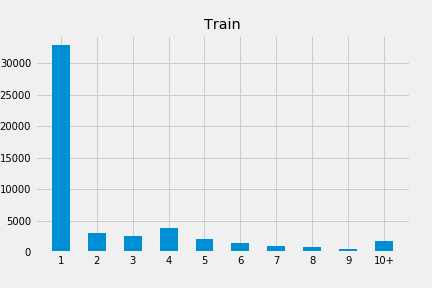
\includegraphics[width=7cm]{figures/train.png} 
\caption{Histogram of distance between the indices of subject and verb in the training dataset. The distribution in the test and the development datasets is similar.}
\end{figure}

With the observation in our pocket, we designed a few simple experiments to get intuition how much the incorrect number agreement can be attributed to the inability of the model to recognize the head of the syntactic subject.

\subsection*{(b) 2. Empirical Experiments} We took the setup from Question 3 as a baseline (\textit{A}) and designed three additional experiments (\textit{B}, \textit{C} and \textit{D}). The experiments varied the length and the difficulty of \textit{training} input. 

Please note that regardless of varied \textit{training} strategies, all models were \textit{evaluated} under the same conditions, as specified in Question 3 for the number prediction task with the exception of training to 25 epochs.

Experiment \textit{A}, baseline, uses all words from the beginning of the sentence up until the position of the verb index. Experiment \textit{B} uses the words from the subject index (inclusive) until the verb index. We expected this experiment to achieve better accuracy than A as we removed the words at the start of the sentence which could disrupt the prediction. In Experiment \textit{C}, we tested how well the network will do if we just give it a noun, the subject, and ask it to predict whether it is plural or singular. In that experiment, the RNN functioned as a feed-forward network. We expected this experiment to yield the best predictions. Finally, for \textit{D}, we wondered if training on \textit{difficult} sentences only, defined as sentences in which the subject and the verb are at least 5 words apart, the learned weights will generalize well to the overall dataset, in which subject and verb are typically adjacent.

\begin{figure}[h]
\centering
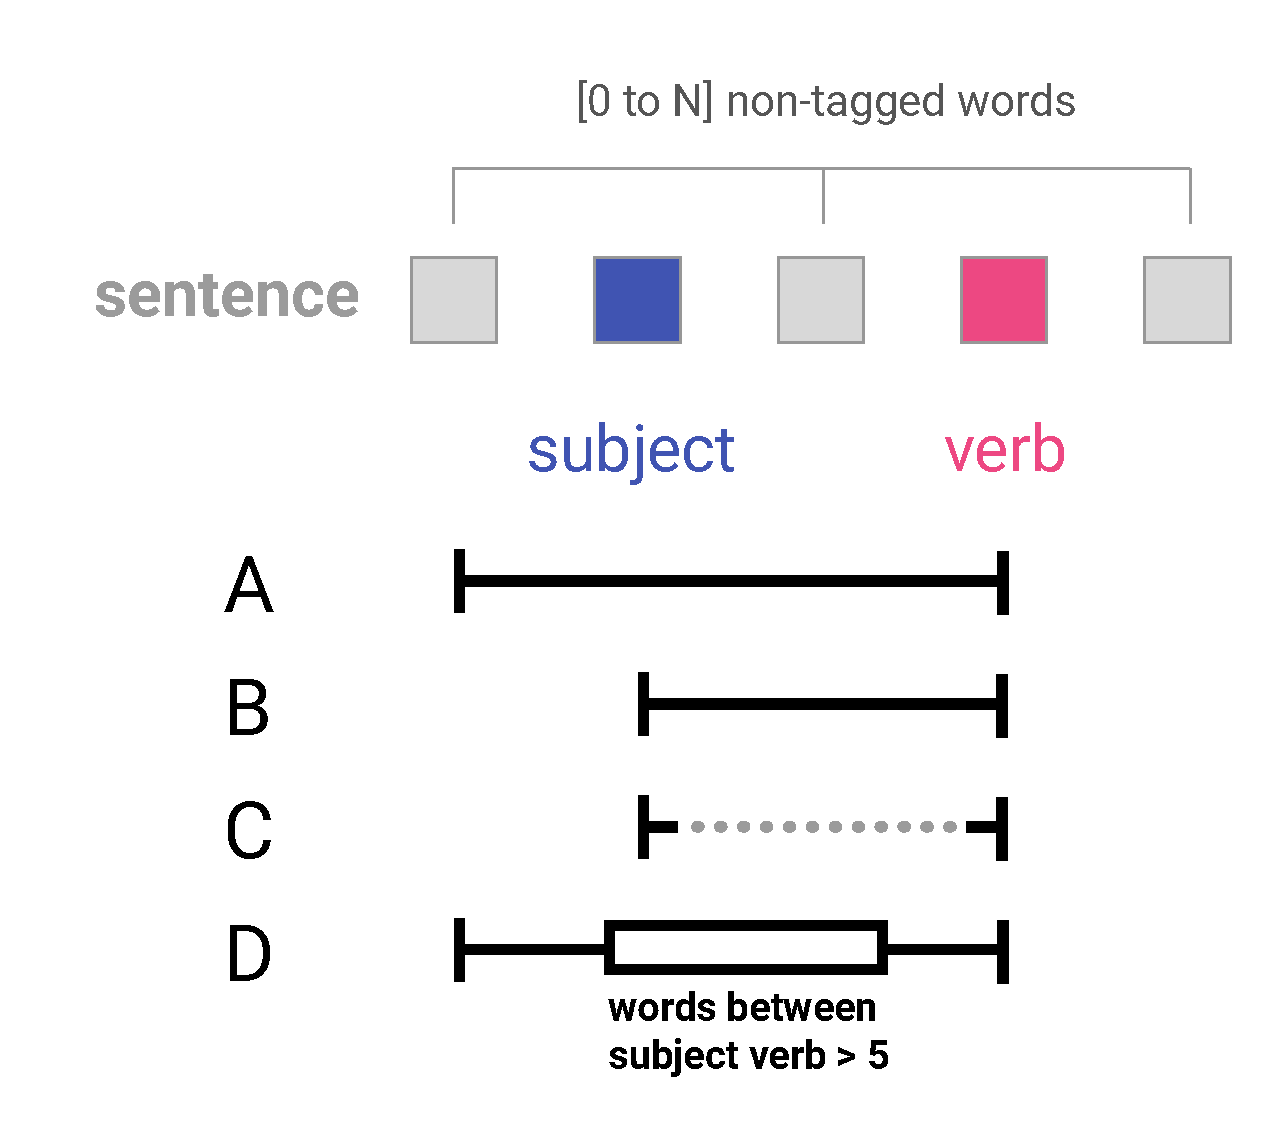
\includegraphics[width=6cm]{figures/window.pdf}
\caption{Experiment word window context length comparison}
\end{figure}

\begin{description}
\item[Length of Training Context:]
\item[Exp. \textbf{A}] All words prior the verb
\item[Exp. \textbf{B}] All words between subject and verb (incl. subject)
\item[Exp. \textbf{C}] Subject only
\item[Exp. \textbf{D}] All words prior the verb. However, only \textit{difficult} sentences were used for training, that is where subject and verb are separated by 3 or more words
\end{description}


\subsection*{(b) 3. Results}

This section summarizes the loss and accuracy which we achieved at each experiment, after hyper-parameter optimization and final training on the best combinations.


\begin{table}[h!]
\begin{center}
\begin{scriptsize}
\begin{tabular}{lrrrr}
\hline
\abovespace\belowspace
Metric & A & B & C & D \\
\hline
\abovespace
Accuracy (pct.) & 88.5 & 82.4 & 79.1 & 71.6 \\
Best Loss & 0.278 & 0.444 & 0.464 & 0.601 \\
\hline
\end{tabular}
\end{scriptsize}
\caption{Evaluation results from the four experiments on the test dataset.}
\end{center}
\end{table}

To our surprise, model \textit{A} scored best, as we had expected superior performance from \textit{B}. Reflecting back, we suspect that \textit{B} underperformed because it learned naively to agree the verb with the first word in the context. During evaluation that was often but not always the case, so \textit{A} generalized better. We see similar loss and accuracy in experiments \textit{C} and \textit{B}. Experiment \textit{D} was arguably the most difficult. We provided the network with only sentence examples of increased difficulty in inspiration of the approach by Linzen \citep{Linzen:2016ud}, but were unable to replicate their results of accuracy increase due to over-sampling of difficult cases.

Lastly, we  wanted to get intuition what the data looks like and how easily separable it is. We visualized the weights learned by the hidden layer by activating it with 1000 samples and then reducing dimensionality to two 'principal components.' We opted for t-SNE rather than other dimensionality reduction approaches such as PCA and SVD because of t-SNE's nonlinearity which plots in low dimensions more realistically the true distance of data-points.
\citep{vanderMaaten:2008tm}.

\begin{figure}[h!]
\centering
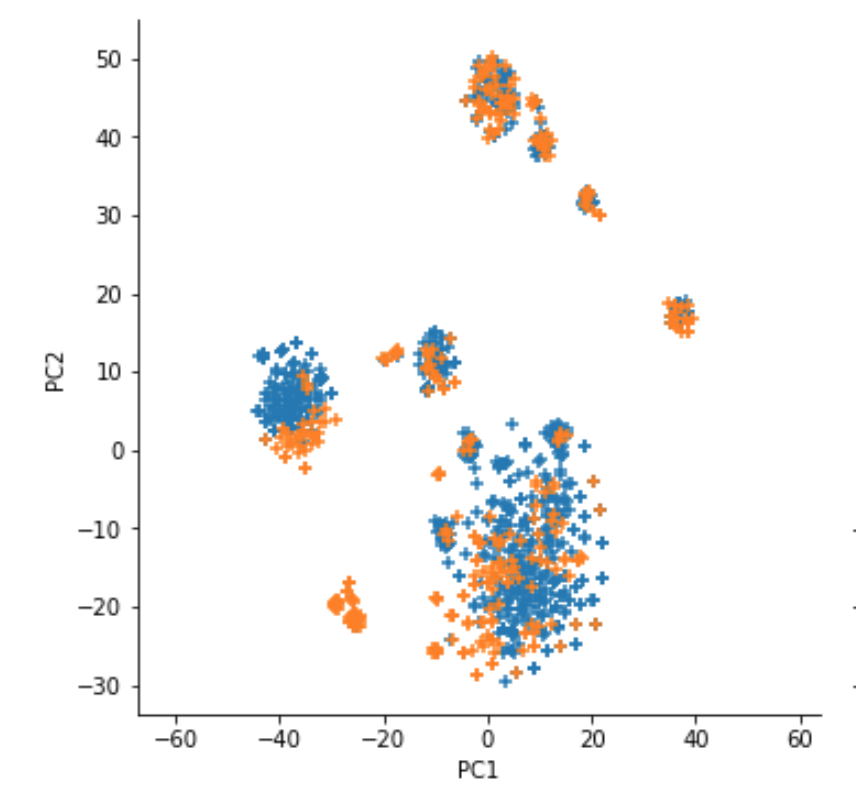
\includegraphics[width=7cm]{figures/t-SNE_activations_of_hidd_layer_on_direct.png} 
\caption{t-SNE activations of the hidden layer in Experiment C. The red and orange labels indicate the true number of the verb, VBZ or VBP. We notice several clusters and speculate that they may correspond to number of words separating the verb from the subject in the data. The model clearly misclassifies the verb number of the sentences clustered in top right, while we see two larger blobs in the center bottom and middle left which can be . The plots from the other experiments did not look too dissimilar so we are not including them with this report.}
\end{figure}


\subsection*{(b) 4. Limitations}
\begin{enumerate}[(i)]
\item \textit{Subject always proceeds verb in the dataset}. We noticed that our dataset has been filtered to include sentences in which the subject always precedes the verb. That ordering tends to be the norm but it is not always the case in the English language, i.e. questions or inverted sentences. In those scenarios, a RNN which looks for context prior to the verb only does not learn enough information to correctly predict a verb's plurality. In the \textbf{Next Steps} section we propose bi-directional recurrent neural networks as one possible remedy.
\item \textit{Verb is always presented in last position}. In a grammar correction application, the network would need to learn to spot subject-verb disagreement without a tagged subject or verb. This extends the current problem definition. One possible ensemble solution can incorporate a Part-of-Speech Tagger (POT) to find the root of the sentence which will support our architecture.
\end{enumerate}
\subsection*{(b) 5. Next Steps}
\begin{enumerate}[(i)]
\item Bi-directional recurrent neural networks (BRNN) could be an extension of the architecture implemented in this coursework. A BRNN is unique in that it can capture context in a backward fashion, as illustrated in Figure 4.    

\begin{figure}[h]
\centering
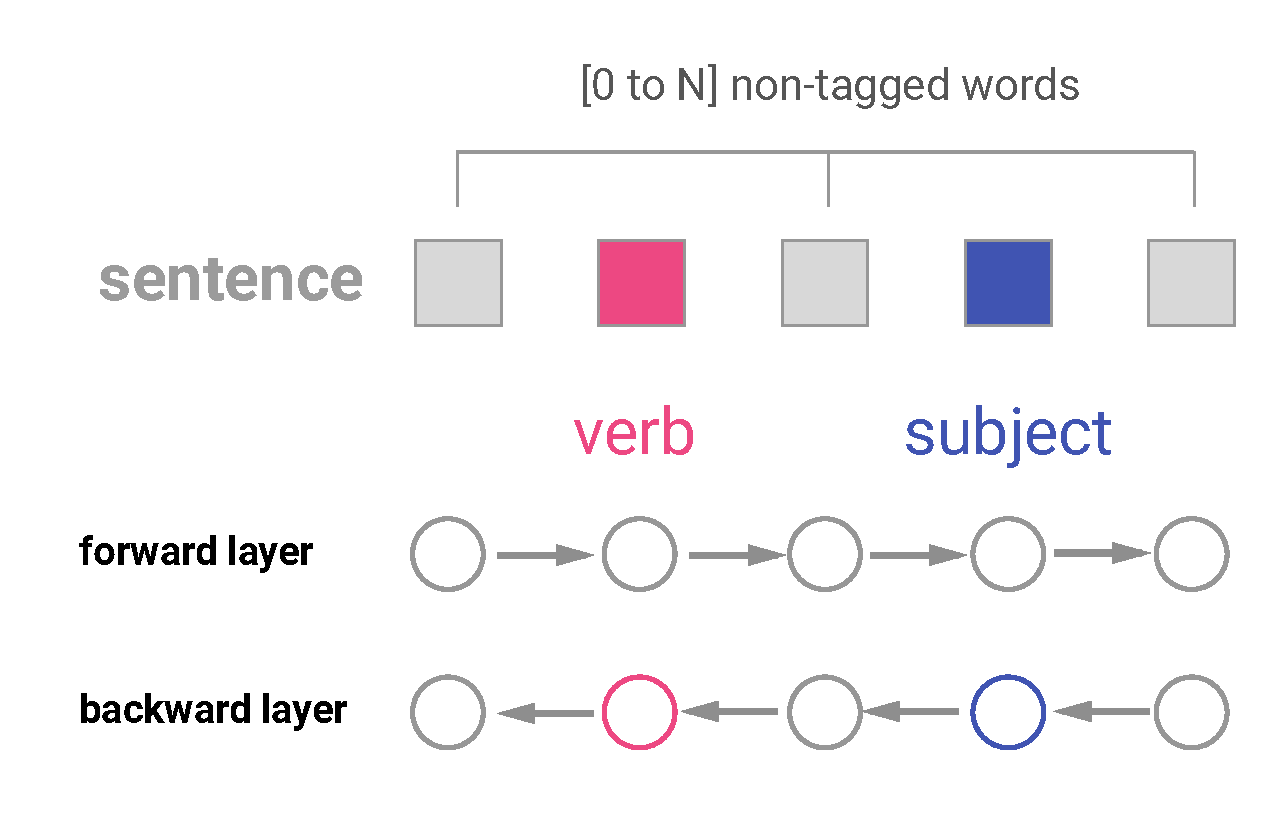
\includegraphics[width=6cm]{figures/birnn.pdf} 
\caption{BRNN layer structure where the backward layer can represent subject post verb.}
\end{figure}

\item Long short-term memory networks (LSTM) are also known to be outperforming recurrent neural networks in grammar learning tasks \citep{Linzen:2016ud}. A RNN is not able to hold a longer context as gradients of previous time steps quickly vanish. An LSTM's gated cell state structure allows for information to pass further down the sentence. 
\end{enumerate}

\newpage
\bibliography{library}
\bibliographystyle{icml2018}

\newpage
\appendix

\end{document}


% This document was modified from the file originally made available by
% Pat Langley and Andrea Danyluk for ICML-2K. This version was created
% by Iain Murray in 2018. It was modified from a version from Dan Roy in
% 2017, which was based on a version from Lise Getoor and Tobias
% Scheffer, which was slightly modified from the 2010 version by
% Thorsten Joachims & Johannes Fuernkranz, slightly modified from the
% 2009 version by Kiri Wagstaff and Sam Roweis's 2008 version, which is
% slightly modified from Prasad Tadepalli's 2007 version which is a
% lightly changed version of the previous year's version by Andrew
% Moore, which was in turn edited from those of Kristian Kersting and
% Codrina Lauth. Alex Smola contributed to the algorithmic style files.

